\documentclass[10pt]{article}
\usepackage{longtable}
\usepackage{float}
\usepackage{wrapfig}
\usepackage{rotating}
\usepackage[normalem]{ulem}
\usepackage{amsmath}
\usepackage{textcomp}
\usepackage{marvosym}
\usepackage{wasysym}
\usepackage{amssymb}
\usepackage{hyperref}
\usepackage{color,soul} % for highlighting
\usepackage{graphicx}
\graphicspath{{/Users/benjaminbass/seacloud/class/earthMaterials/picBank/}}

\usepackage{frame,color}
\usepackage{framed}
\usepackage{minibox}

% \usepackage[T1]{fontenc}
% \usepackage{tilting} %bring title up
% \setlength{\droptitle}{-10cm}

\usepackage[version=3]{mhchem}
% How to Use MChem
% \ce{SO4^2-}
% \ce{^{227}_{90}Th+}
% \ce{A\bond{-}B\bond{=}C\bond{#}D}
% \ce{CO2 + C -> 2CO}
% \ce{SO4^2- + Ba^2+ -> BaSO4 v}


\author{Benjamin Bass}
\date{15 March 2016}
\title{\vspace{-2.0cm}Zircon} %bring title up temporary Fix

\begin{document}

\maketitle

% \framebox{Use frameboxes until figure out alignmen}

\begin{center}
  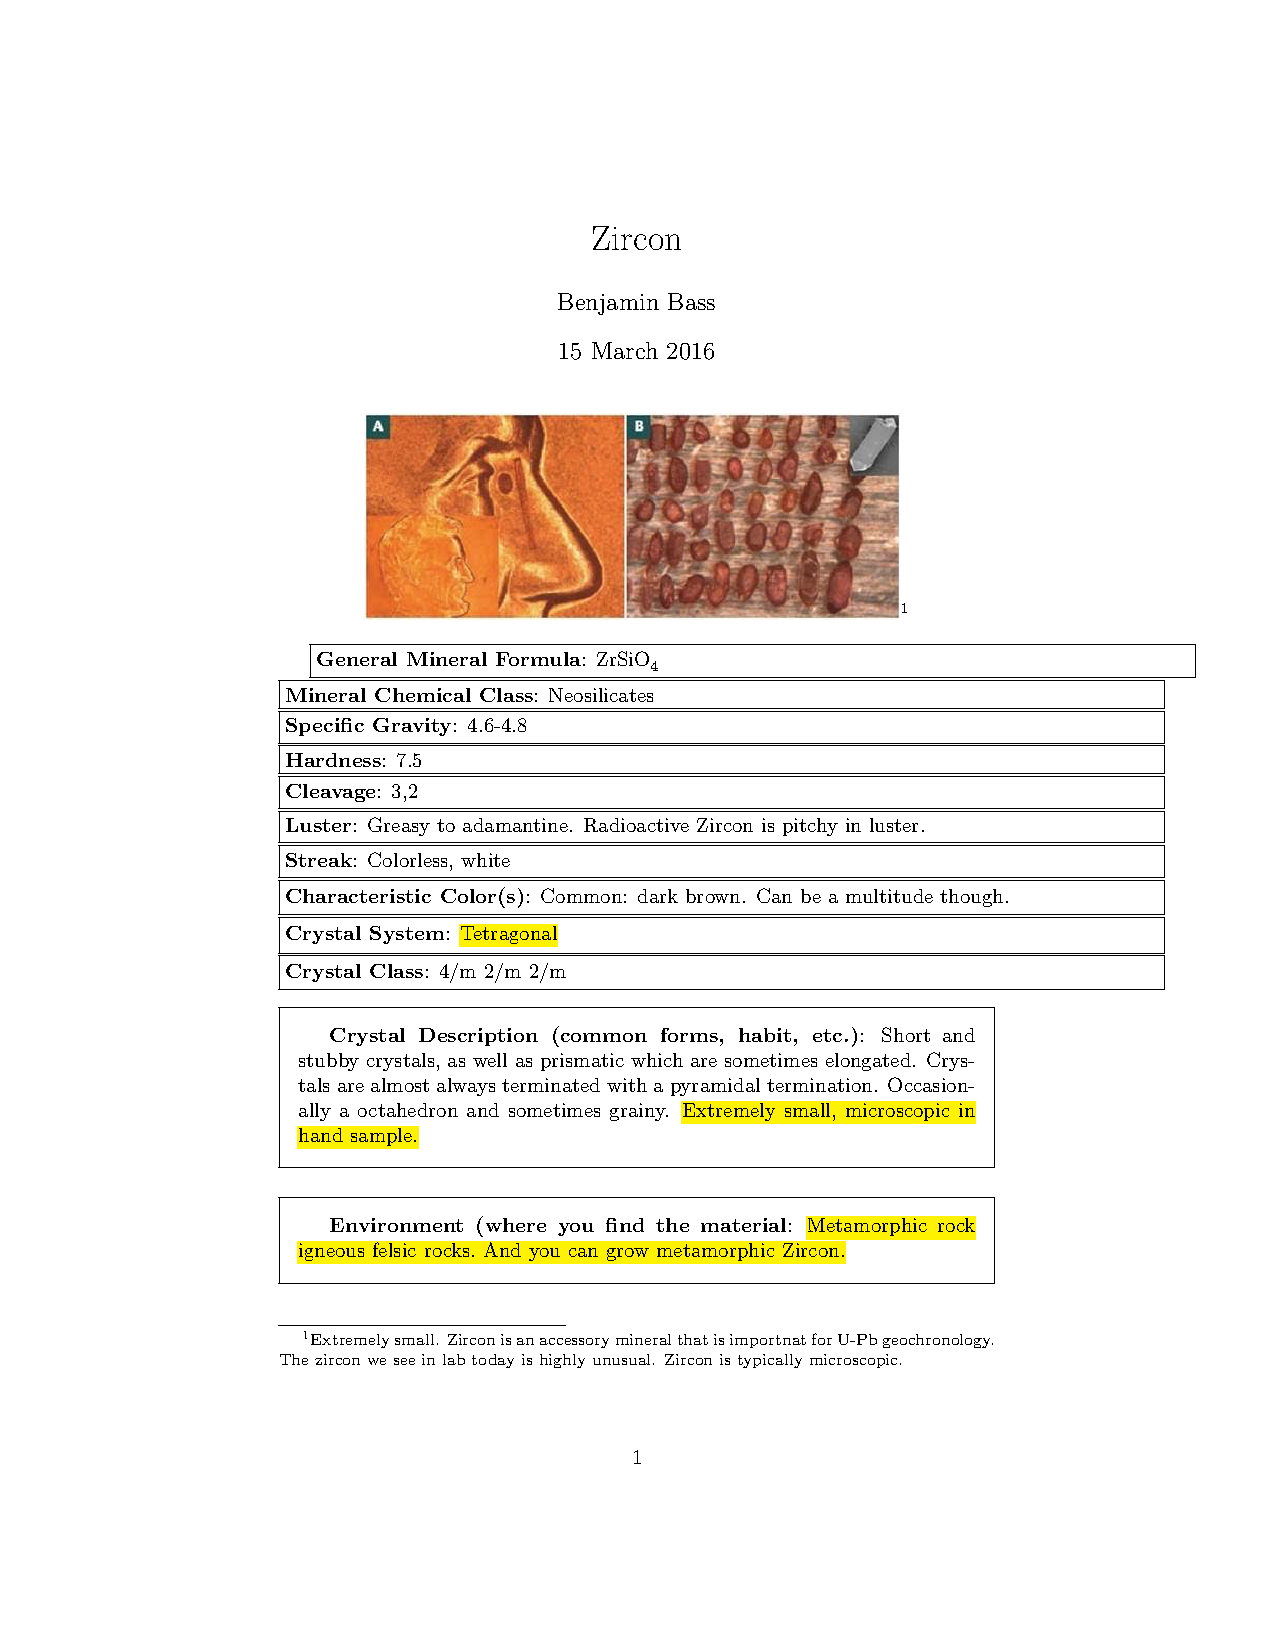
\includegraphics[scale=0.5]{zircon}\footnote{Extremely small. Zircon is an accessory mineral that is importnat for U-Pb geochronology. The zircon we see in lab today is highly unusual. Zircon is typically microscopic.}
\end{center}



\framebox[15cm][l]{\textbf{General Mineral Formula}: \ce{ZrSiO4} }\
\framebox[15cm][l]{\textbf{Mineral Chemical Class}: Neosilicates }\
\framebox[15cm][l]{\textbf{Specific Gravity}: 4.6-4.8 }\
\framebox[15cm][l]{\textbf{Hardness}: 7.5 }\
\framebox[15cm][l]{\textbf{Cleavage}: 3,2 }\
\framebox[15cm][l]{\textbf{Luster}: Greasy to adamantine. Radioactive Zircon is pitchy in luster. }\
\framebox[15cm][l]{\textbf{Streak}: Colorless, white }\
\framebox[15cm][l]{\textbf{Characteristic Color(s)}: Common: dark brown. Can be a multitude though.  }\
\framebox[15cm][l]{\textbf{Crystal System}: \hl{Tetragonal} }\
\framebox[15cm][l]{\textbf{Crystal Class}: 4/m 2/m 2/m  }\

\begin{framed}
  \textbf{Crystal Description (common forms, habit, etc.)}: Short and stubby crystals, as well as prismatic which are sometimes elongated. Crystals are almost always terminated with a pyramidal termination. Occasionally a octahedron and sometimes grainy. \hl{Extremely small, microscopic in hand sample.}
\end{framed}

\begin{framed}
  \textbf{Environment (where you find the material}: \hl{Metamorphic rock
igneous felsic rocks. And you can grow metamorphic Zircon.}
\end{framed}

\begin{framed}
  \textbf{Common Mineral Associations (in samples, also consult text, notes}: Albite, Quartz, Biotite, Chlorite.
\end{framed}

\begin{framed}
  \textbf{Scientific Usage/Significance}: Uranium-Lead dating all the way to lead. Use the ratio of uranium to lead in order to tell how long it has been there. Our principle method of really old dating. Zircon is an accessory mineral that is importnat for U-Pb geochronology. The zircon we see in lab today is highly unusual. Zircon is typically microscopic.
\end{framed}

\begin{framed}
  \textbf{Industrial or Social Use/Significance}: Used in nuclear reactors. Also as a foundry in brick.
\end{framed}

\begin{framed}
  \textbf{Environmental Significance}: Does not break down easily. Can be found in lots of places. A source of metals as well.
\end{framed}

% Possible other Solutions
% \framebox(300,20){\minibox{\textbf{R-Sq}:For example}}

\end{document}
%%% Local Variables:
%%% mode: latex
%%% TeX-master: t
%%% End:
